%
% intgration.tex
%
% Copyright (C) 2021 by SpaceLab.
%
% Flatsat Platform Documentation
%
% This work is licensed under the Creative Commons Attribution-ShareAlike 4.0
% International License. To view a copy of this license,
% visit http://creativecommons.org/licenses/by-sa/4.0/.
%

%
% \brief Modules Integration and Testing chapter.
%
% \author João Cláudio Elsen Barcellos <joaoclaudiobarcellos@gmail.com>
%
% \institution Universidade Federal de Santa Catarina (UFSC)
%
% \version 0.2.0
%
% \date 2021/06/15
%

\chapter{Modules Integration and Testing} \label{ch:modules-integration-and-testing}

The CubeSat that will be used in the FloripaSat-2 consists mainly of three modules, OBDH, TTC and EPS, which are the core of the CubeSat, and payloads. In order to facilitate the integration and testing of all these subsystems a methodology had to be created, which will be done using the FlatSat platform.

This process was divided in five steps, which will be presented in the next sections with more details. First, the core of the CubeSat will be connected together, to evaluate the interaction between them. Then, the GRS will be emulated to verify if there will be no errors in data transmission and reception. Later, all payloads will be connected together with the core of the CubeSat to evaluate their behavior. Next the the GRS will be emulated again with the core and payloads integrated, considering the data transmission from the payloads. Finally, a long term test will be made.

\section{Testing the CubeSat Core}

In this step, the interaction between OBDH, EPS and TTC will be evaluated. Therefore, the main communication protocols that these three modules use to interact will be tested. The deployment sequence will be performed with a fully functional EPS and also with a partially functional EPS, to search for critical errors. Subsequently, the operation of these modules will be evaluated.

\subsection{Experiment Setup}
\label{subsec:experiment-setup-1}

First, all three modules will be connected to the FlatSat. The EPS needs to be connected to \textbf{Slot 1}, and the other two modules can be connected in any slots, like in figure \ref{fig:connections-1}.

\begin{figure}[H]
	\begin{center}
		
\includegraphics[width=0.5\textwidth]{figures/dummy-image.png}
		\caption{OBDH, EPS and TTC connected in the FlatSat platform.}
		\label{fig:connections-1}
	\end{center}
\end{figure}

Still with the kill-switches cutting-off the power supply for the EPS, a power supply is connected to the Battery Module, like in figure \ref{fig:connections-2}. But, if the EPS won't be used in the experiment, OBDH and TTC can be powered by using an external power supply connected to the binding posts CN10 or CN4. Jumpers are used to connect their respective PC-104 power supply pins to CN12 or CN6, like in figure \ref{fig:connections-3}. 

\begin{figure}[H]
	\begin{center}
		
\includegraphics[width=0.5\textwidth]{figures/dummy-image.png}
		\caption{Setup using the EPS and Battery Module.}
		\label{fig:connections-2}
	\end{center}
\end{figure}

\begin{figure}[H]
	\begin{center}
		
\includegraphics[width=0.5\textwidth]{figures/dummy-image.png}
		\caption{Setup without the EPS and Battery Module.}
		\label{fig:connections-3}
	\end{center}
\end{figure}

A launchpad will emulate the antennas, like the MSP-EXP430F5529LP. Then, this launchpad can be connected in the \textbf{Slot 7}, so OBDH and TTC can communicate with it, like in figure \ref{fig:connections-4}.

\begin{figure}[H]
	\begin{center}
		
\includegraphics[width=0.5\textwidth]{figures/dummy-image.png}
		\caption{Launchpad emulating the Antenna Module.}
		\label{fig:connections-4}
	\end{center}
\end{figure}

\subsection{Deployment Sequence}

After the decouple of the satellite from its deployer in orbit, the kill-switches will be released and will enable the power supply of the core modules. The EPS will distribute energy for all subsystems, with the Battery Module coupled, composed by four lithium-ion 18650 cells. After the boot, OBDH waits 45 minutes before operating normally. Then, the OBDH will act to deploy the antennas. Similarly to the ODBH, after de boot, TTC waits 55 minutes before operating normally. Redundantly, the TTC will also act to deploy the antennas. The TTC will enable the sub-modules Downlink/Uplink and Beacon at the end of the process. Every 12 hours, this process repeats, indefinitely, but the OBDH and TTC don’t need to wait anymore to operate normally. The figure \ref{fig:deployment-flowchart} shows the process described.

\begin{figure}[H]
	\begin{center}
		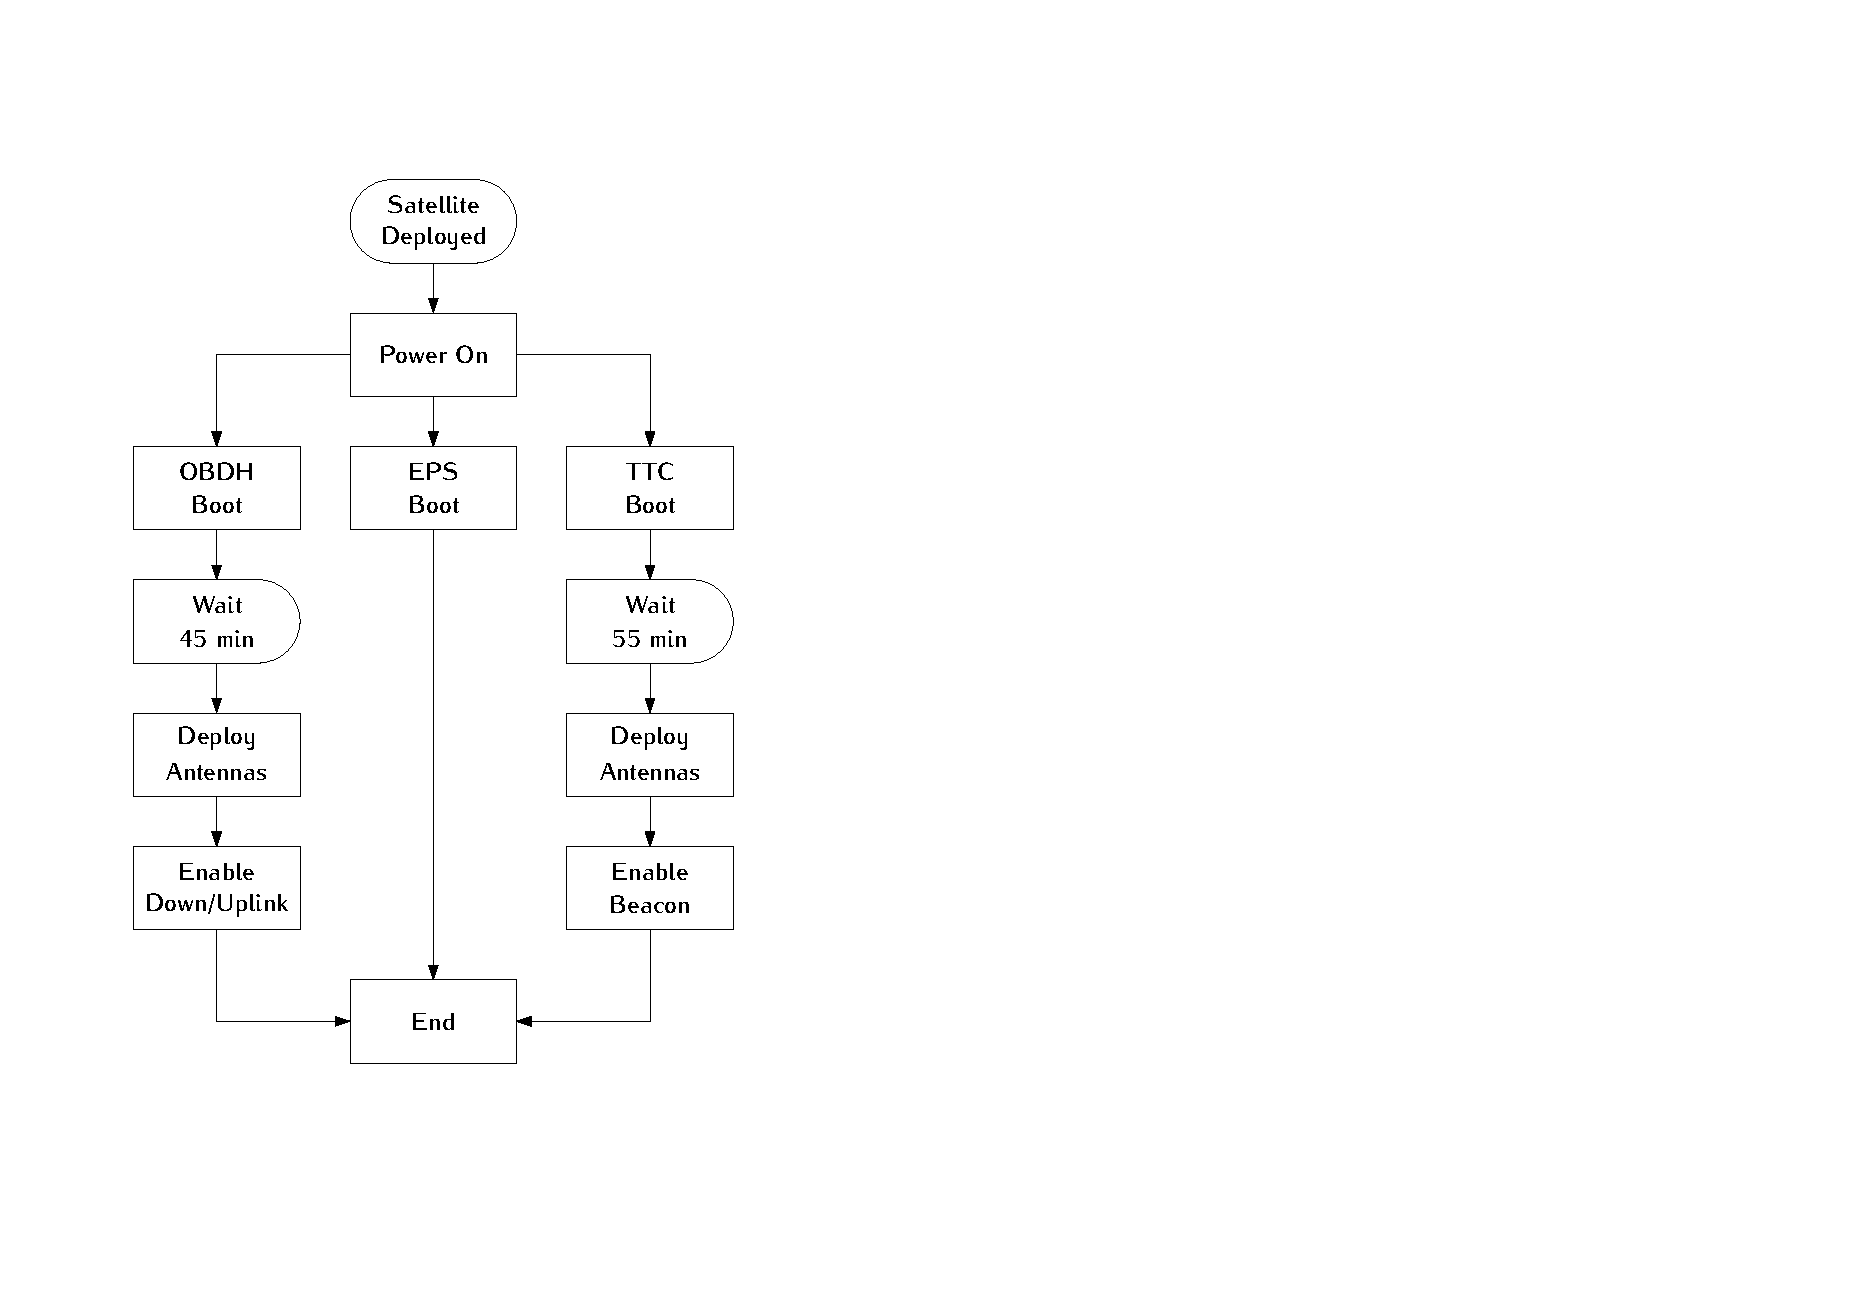
\includegraphics[width=0.5\textwidth]{figures/deployment-flowchart.pdf}
		\caption{Flowchart of the deployment sequence.}
		\label{fig:deployment-flowchart}
	\end{center}
\end{figure}

\subsubsection{Waiting Time and Redudancy}

The OBDH and TTC won’t operate normally for 45 minutes and 55 minutes, respectively. The validation criteria for this first experiment is shown in the table \ref{tab:validation-criteria-1}.

\begin{table}[H]
	\centering
	\resizebox{\columnwidth}{!}{\begin{tabular}{cc}
		\toprule[1.5pt]
		\textit{Question} & \textit{Answer} \\
		\midrule
		Is the OBDH doing something before 45 minutes?  & No, 45 minutes elapsed before the OBDH act to deploy the antennas. \\
		Is the TTC doing something before 55 minutes? & No, 55 minutes elapsed before the TTC act to deploy the antennas. \\
		\bottomrule[1.5pt]
	\end{tabular}}
	\caption{Validation criteria.}
	\label{tab:validation-criteria-1}
\end{table}

Then, OBDH and TTC, respectively, will act to deploy the antennas. The validation criteria for this first experiment is shown in the table \ref{tab:validation-criteria-2}.

\begin{table}[H]
	\centering
	\resizebox{\columnwidth}{!}{\begin{tabular}{cc}
			\toprule[1.5pt]
			\textit{Question} & \textit{Answer} \\
			\midrule
			TTC was capable of doing the deployment of the antennas, like the OBDH? & Yes, OBDH and TTC were capable of doing the same thing.\\
			\bottomrule[1.5pt]
	\end{tabular}}
	\caption{Validation criteria.}
	\label{tab:validation-criteria-2}
\end{table}

\subsubsection{Power Supply}

The EPS uses the MPPT, a method used to distribute energy with more efficiency. But, if the EPS cannot implement this method, theoretically, still would be able to distribute the energy to the other modules, but with less efficiency. But, to guarantee, this need to be evaluated. The validation criteria for this first experiment are shown in the table \ref{tab:validation-criteria-3}.

\begin{table}[H]
	\centering
	\resizebox{\columnwidth}{!}{\begin{tabular}{cc}
			\toprule[1.5pt]
			\textit{Question} & \textit{Answer} \\
			\midrule
			If the EPS fails to implement the MPPT, OBDH and TTC will boot? & Yes, OBDH and TTC booted.\\
			\bottomrule[1.5pt]
	\end{tabular}}
	\caption{Validation criteria.}
	\label{tab:validation-criteria-3}
\end{table}

\subsection{Interactions}

After the deployment sequence, during 12 hours, the satellite works normally. Therefore, the modules will get all the relevant data for the mission. This data flows between modules, via UART, SPI and $I^{2}C$. These interactions need to be evaluated to understand if the data is traveling correctly, with no faults. 

\subsubsection{Interaction between TTC and EPS}

The sub-module Beacon interacts with the EPS using the UART. Every one minute the EPS will receive a request, from the sub-module Beacon, to send data. If the data sent from the EPS is valid, the Beacon will transmit the data from the TTC itself and from the EPS. Otherwise, only the data from TTC will be transmitted. This operation is presented in figure \ref{fig:beacon-flowchart}.  

\begin{figure}[H]
	\begin{center}
		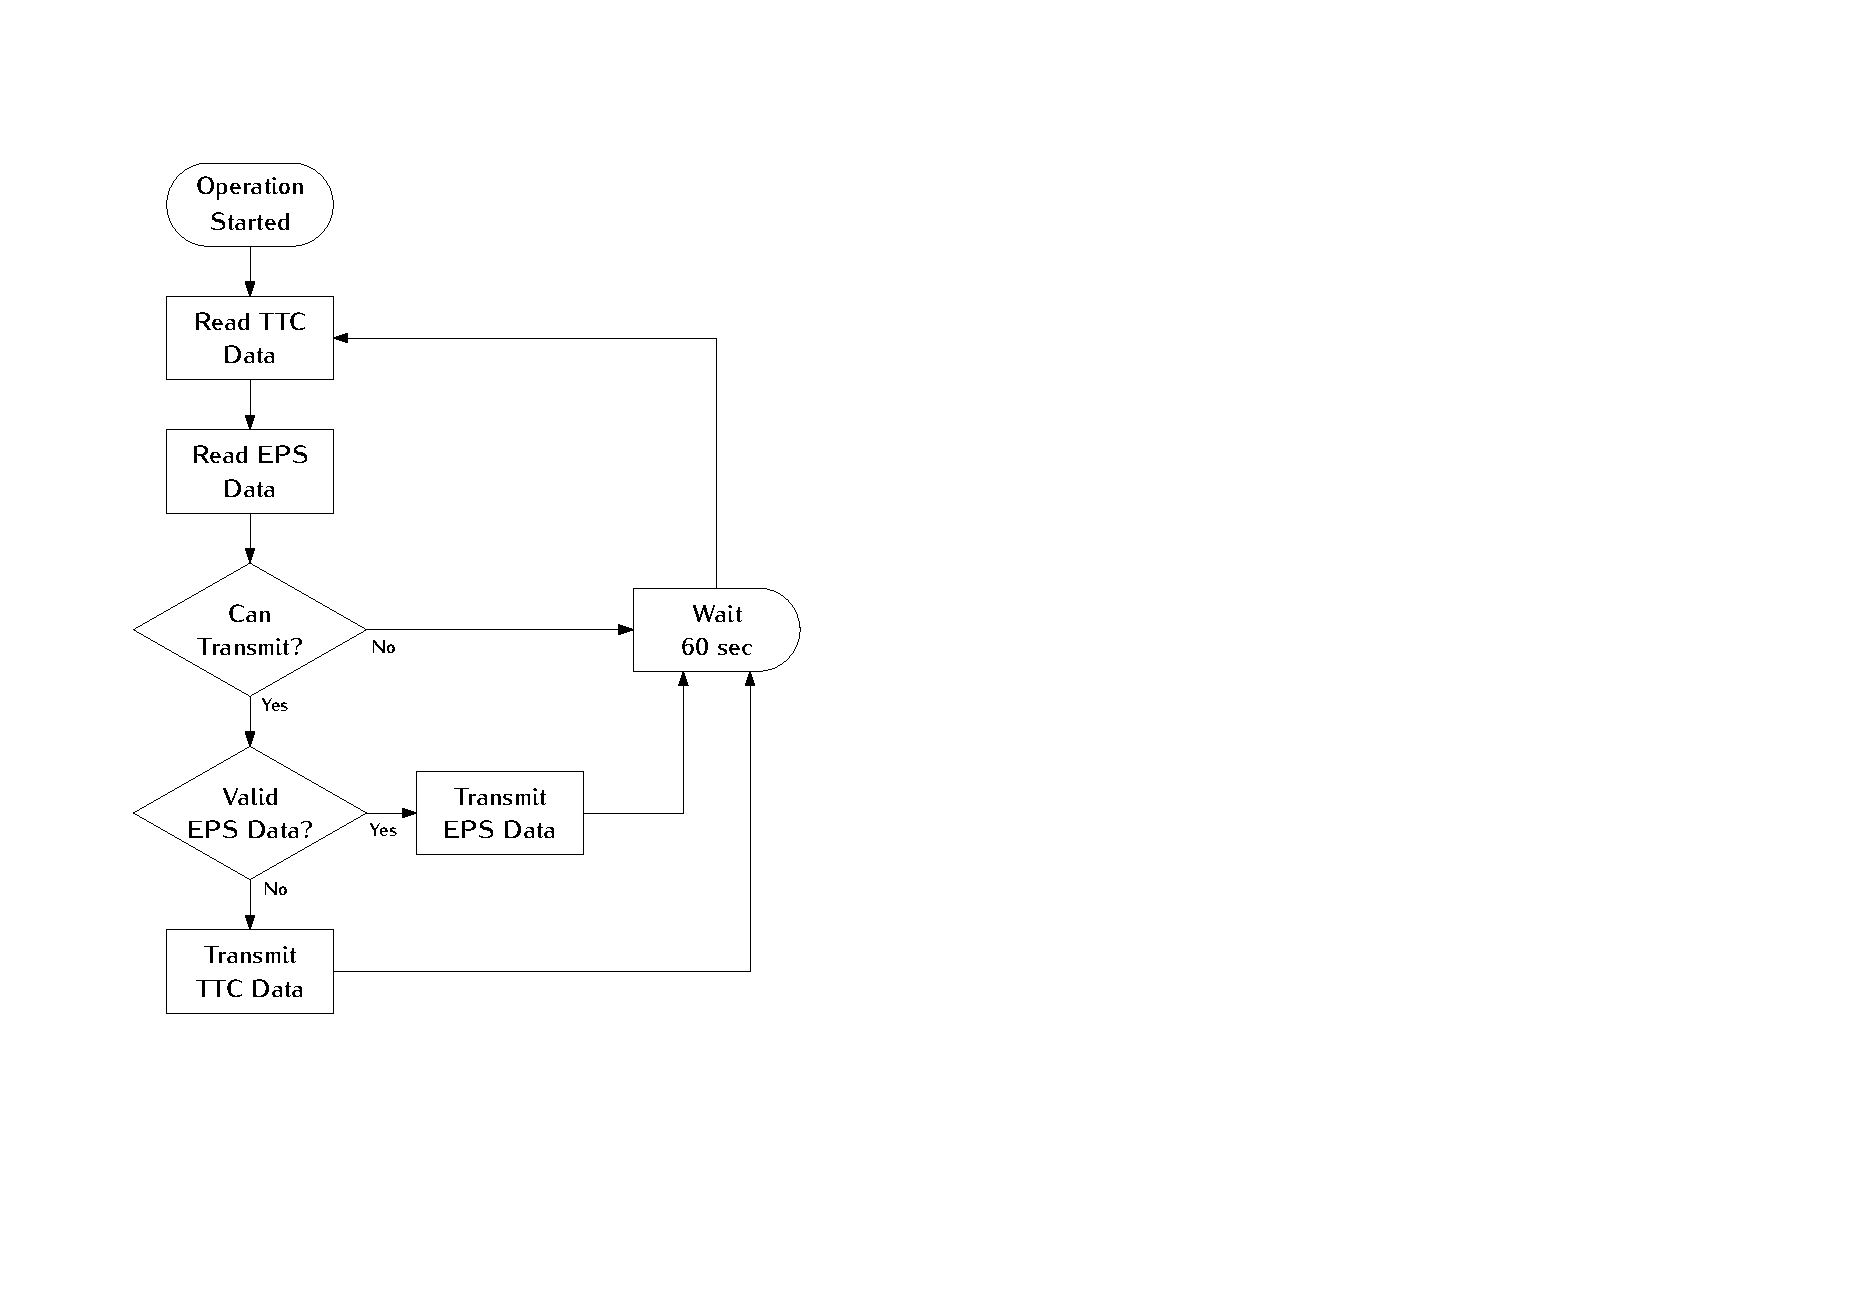
\includegraphics[width=0.5\textwidth]{figures/beacon-flowchart.pdf}
		\caption{Flowchart of the Beacon operation.}
		\label{fig:beacon-flowchart}
	\end{center}
\end{figure}

In the firmware of each module, it is calculated the checksum of every message that is transmitted or received. This way, it is possible to understand if the message sent from one module is the same that is received from the other. This will be used to validate the interaction between EPS and Beacon. The validation criteria is shown in table \ref{tab:validation-criteria-4}. 

\begin{table}[H]
	\centering
	\resizebox{\columnwidth}{!}{\begin{tabular}{cc}
			\toprule[1.5pt]
			\textit{Question} & \textit{Answer} \\
			\midrule
			EPS received the same message that was sent from Beacon? & Yes, the checksum was equal in both ends.\\
			Beacon received the same message that was sent from EPS? & Yes, the checksum was equal in both ends.\\
			If the data from EPS is invalid, just the TTC data is transmitted? & Yes, just the data from TTC is transmitted.\\
			And if it is valid, TTC and EPS data are transmitted? & Yes, both are transmitted.\\
            This interaction occurs every one minute? & Yes, this interaction is periodic.\\

			\bottomrule[1.5pt]
	\end{tabular}}
	\caption{Validation criteria.}
	\label{tab:validation-criteria-4}
\end{table}

\subsubsection{Interaction between OBDH with EPS and TTC}

The OBDH interacts with the TTC using SPI and with the EPS using $I^{2}C$. Every one minute, the EPS and TTC will receive a request, from the OBDH, to send data. Then, the OBDH will save all the received data (
including the data from the OBDH itself) in memory. This operation is presented in figure \ref{fig:obdh-flowchart}. 

\begin{figure}[H]
	\begin{center}
		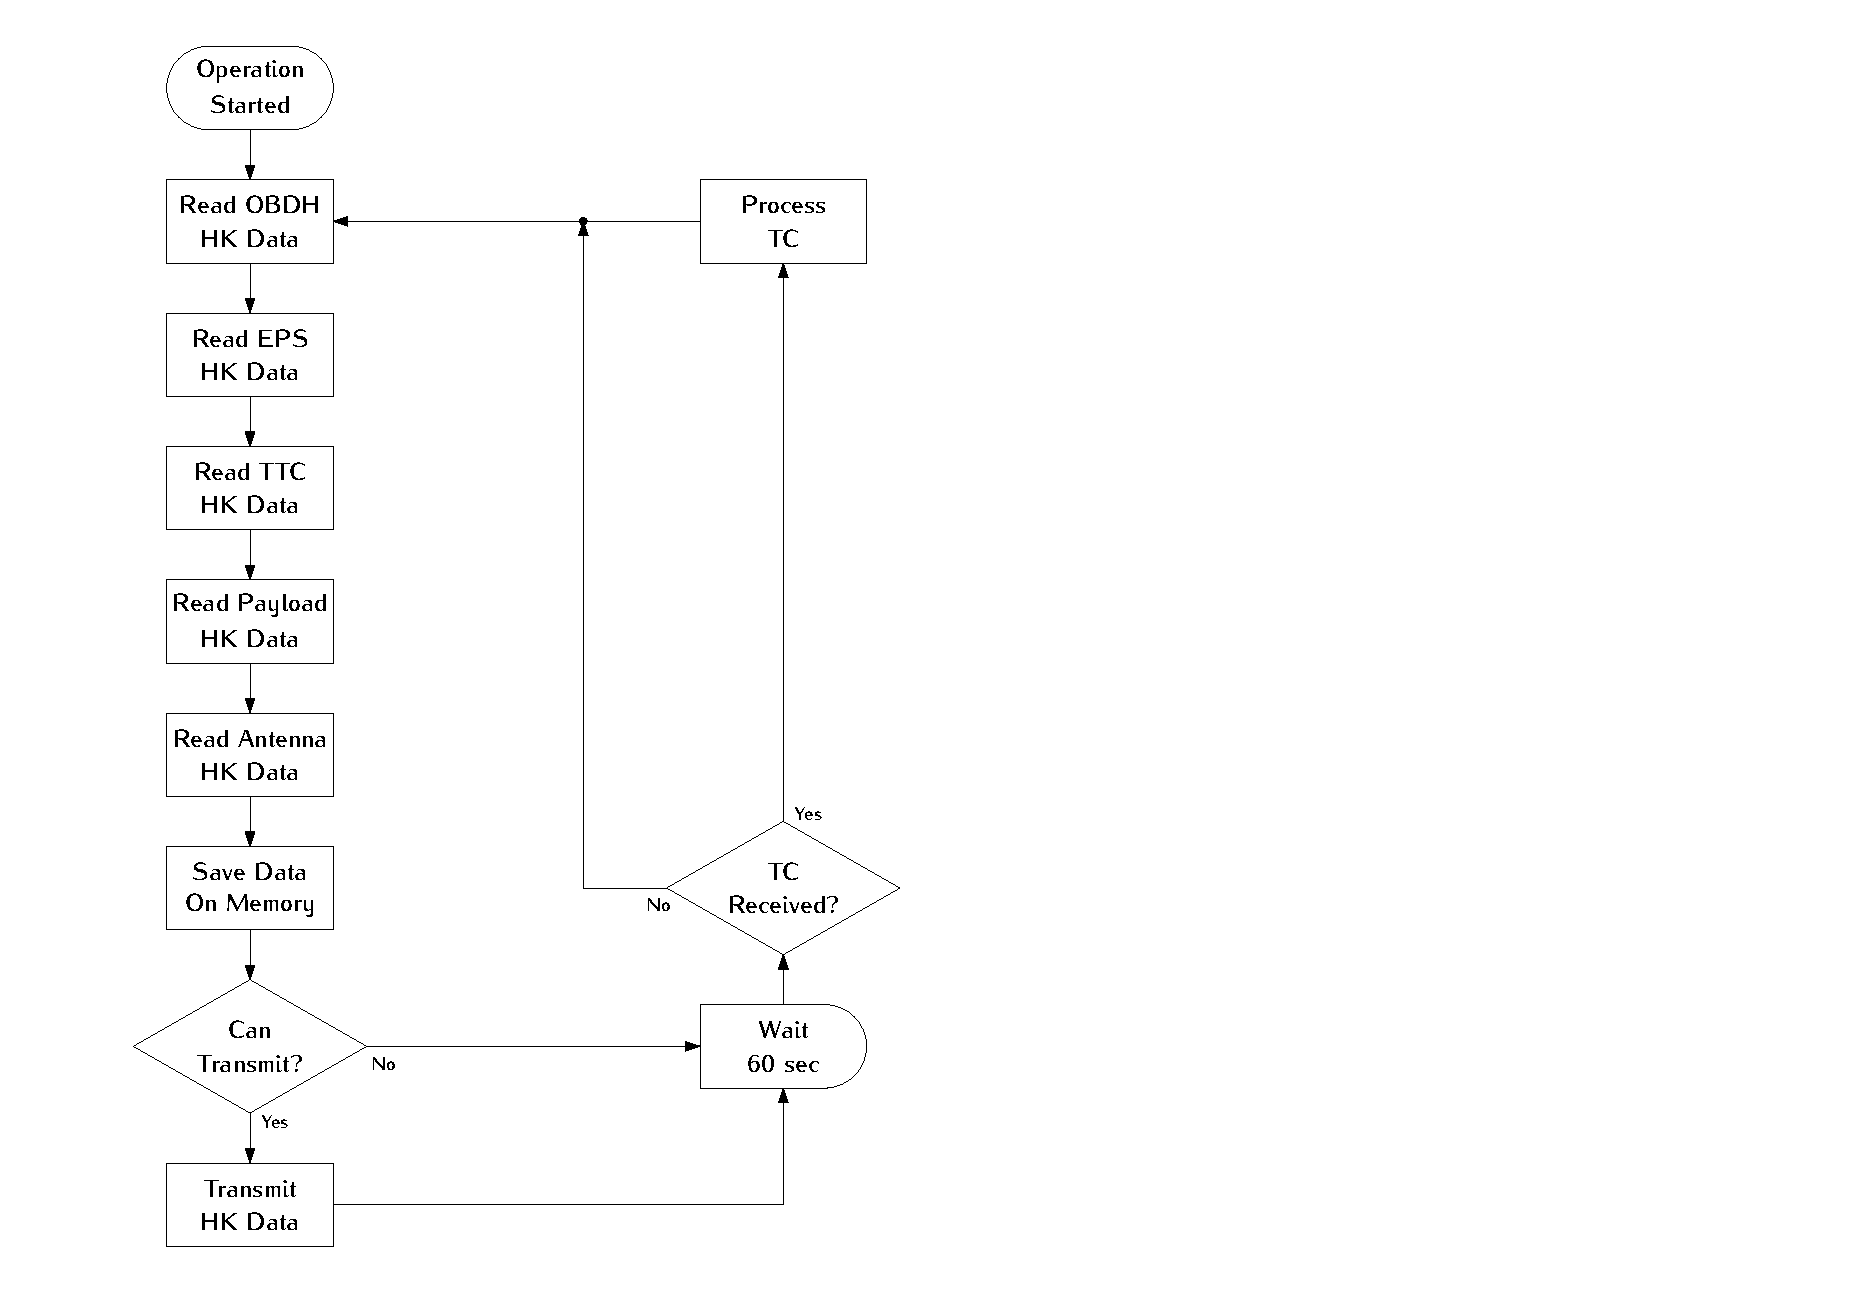
\includegraphics[width=0.5\textwidth]{figures/obdh-flowchart.pdf}
		\caption{Flowchart of the Beacon operation.}
		\label{fig:obdh-flowchart}
	\end{center}
\end{figure}

As said before, the checksum in both ends will be compared to define if the messages are being correctly sent and received. The validation criteria is shown in table \ref{tab:validation-criteria-5}.

\begin{table}[H]
	\centering
	\resizebox{\columnwidth}{!}{\begin{tabular}{cc}
			\toprule[1.5pt]
			\textit{Question} & \textit{Answer} \\
			\midrule
			EPS received the same message that was sent from OBDH? & Yes, the checksum was equal in both ends.\\
			OBDH received the same message that was sent from EPS? & Yes, the checksum was equal in both ends.\\
			TTC received the same message that was sent from OBDH? & Yes, the checksum was equal in both ends.\\
			OBDH received the same message that was sent from TTC? & Yes, the checksum was equal in both ends.\\
			OBDH was capable of saving all the data? & Yes, all data was saved in memory.\\
            This interactions occurs every one minute? & Yes, this interactions are periodic.\\

			\bottomrule[1.5pt]
	\end{tabular}}
	\caption{Validation criteria.}
	\label{tab:validation-criteria-5}
\end{table}

\section{Testing the CubeSat Core with GRS}

In this step, all the interactions between the core modules were validated. Now, the interaction of these modules with the GRS need to be evaluated. To emulate the GRS, a software, the GQRX, will be used with two boards to transmit and receive TC's, the USRP and SDR, respectively. The figure \ref{fig:tc-flowchart} shows all TC's involved.

\begin{figure}[H]
	\begin{center}
		\includegraphics[width=0.4\textwidth]{figures/tc-flowchart.pdf}
		\caption{Flowchart of the telecommand processing.}
		\label{fig:tc-flowchart}
	\end{center}
\end{figure}

\subsection{Experiment Setup}

Similarly to the subsection \ref{subsec:experiment-setup-1}, all three modules will be connected to the FlatSat. But, now, the GRS will be emulated. The USRP and the SDR should be connected to the computer, witch will be running the GQRX, like in figure \ref{fig:connections-5}.

\begin{figure}[H]
	\begin{center}
		
\includegraphics[width=0.5\textwidth]{figures/dummy-image.png}
		\caption{Setup to emulate the GRS.}
		\label{fig:connections-5}
	\end{center}
\end{figure}

\subsection{Receiving data from GRS}

As shown in figure \ref{fig:obdh-flowchart}, after OBDH saves the data in memory, it will check if TC's were received, then, it will process the TC's. In figure \ref{fig:tc-flowchart}, are listed all the TC's that can be processed. In this step, only the TC's with ID 47h, 48h, 4Bh won't be transmited by GRS, because there aren't payloads connected to the FlatSat. The sub-module Uplink has the function of receiving the TC's and inform OBDH. The GQRX will be used to configure the message that will be transmitted to the Uplink and the USRP should transmit this message to it. The validation criteria is shown in table \ref{tab:validation-criteria-6}.

\begin{table}[H]
	\centering
	\resizebox{\columnwidth}{!}{\begin{tabular}{cc}
			\toprule[1.5pt]
			\textit{Question} & \textit{Answer} \\
			\midrule
			TC with ID 40h was received? & Yes, OBDH was capable of recognising this TC.\\
			TC with ID 41h was received? & Yes, OBDH was capable of recognising this TC.\\
			TC with ID 42h was received? & Yes, OBDH was capable of recognising this TC.\\
			TC with ID 43h was received? & Yes, OBDH was capable of recognising this TC and the hibernation mode was enable.\\
			TC with ID 44h was received? & Yes, OBDH was capable of recognising this TC and the hibernation mode was disable.\\
			TC with ID 45h was received? & Yes, OBDH was capable of recognising this TC.\\
			TC with ID 46h was received? & Yes, OBDH was capable of recognising this TC.\\
			TC with ID 49h was received? & Yes, OBDH was capable of recognising this TC and the memory was erased.\\
			TC with ID 4Ah was received? & Yes, OBDH was capable of recognising this TC and the core modules was reset.\\
			\bottomrule[1.5pt]
	\end{tabular}}
	\caption{Validation criteria.}
	\label{tab:validation-criteria-6}
\end{table}

\subsection{Transmitting data to GRS}

As shown in figure \ref{fig:beacon-flowchart}, the Beacon transmits the data from the EPS and/or TTC, every one minute. The TC's 00h and 01h corresponds to the data of EPS an TTC, respectively. The SDR will receive this TC's and will be possible to see them in the GQRX. The validation criteria is shown in table \ref{tab:validation-criteria-7}.

\begin{table}[H]
	\centering
	\resizebox{\columnwidth}{!}{\begin{tabular}{cc}
			\toprule[1.5pt]
			\textit{Question} & \textit{Answer} \\
			\midrule
			TC with ID 00h was received? & Yes, the message is shown in GQRX.\\
			TC with ID 01h was received? & Yes, the message is shown in GQRX.\\
			TC's are received periodically? & Yes, the message is shown periodically in GQRX.\\
			\bottomrule[1.5pt]
	\end{tabular}}
	\caption{Validation criteria.}
	\label{tab:validation-criteria-7}
\end{table}

But, the sub-module Downlink will transmit TC's to the GRS too. For example, all the feedback transmitted to the GRS, shown in figure \ref{fig:tc-flowchart}, is transmitted by the Downlink. Also, as shown in figure \ref{fig:obdh-flowchart}, after OBDH saves the data, the Downlink will transmit a TC, with the data of all modules, every one minute. Consequently, this TC's will be shown in GQRX too. The validation criteria is shown in table \ref{tab:validation-criteria-8}.

\begin{table}[H]
	\centering
	\resizebox{\columnwidth}{!}{\begin{tabular}{cc}
			\toprule[1.5pt]
			\textit{Question} & \textit{Answer} \\
			\midrule
			In response to the TC with ID 43h, the TC with ID 25h was received? & Yes, the message is shown in GQRX.\\
			In response to the TC with ID 44h, the TC with ID 25h was received? & Yes, the message is shown in GQRX.\\
			In response to the TC with ID 45h, the TC with ID 25h was received? & Yes, the message is shown in GQRX.\\
			In response to the TC with ID 46h, the TC with ID 25h was received? & Yes, the message is shown in GQRX.\\
			In response to the TC with ID 49h, the TC with ID 25h was received? & Yes, the message is shown in GQRX.\\
			In response to the TC with ID 4Ah, the TC with ID 25h was received? & Yes, the message is shown in GQRX.\\
			In response to the TC with ID 40h, the TC with ID 21h was received? & Yes, the message is shown in GQRX.\\
			In response to the TC with ID 41h, the TC with ID 22h was received? & Yes, the message is shown in GQRX.\\
			In response to the TC with ID 42h, the TC with ID 23h was received? & Yes, the message is shown in GQRX.\\
			Every one minute a TC with ID 20h is received? & Yes, the message is shown periodically in GQRX.\\
			\bottomrule[1.5pt]
	\end{tabular}}
	\caption{Validation criteria.}
	\label{tab:validation-criteria-8}
\end{table}
